\documentclass[UTF8]{ctexart}
\usepackage[left=2.50cm, right=2.50cm, top=2.50cm, bottom=2.50cm]{geometry}
\usepackage{amsmath, amsfonts, amssymb}
\usepackage[english]{babel}
\usepackage{graphicx}
\usepackage{url}
\usepackage{bm}
\usepackage{indentfirst}
\usepackage{threeparttable}
\usepackage{multirow}
\usepackage{cite}
% \usepackage{booktabs}
\usepackage{listings}
\usepackage{algorithm}
\usepackage{float}
\usepackage{algorithmic}
\usepackage{inconsolata}
\usepackage{color}
\usepackage{xcolor}
% \usepackage{abstract}
\usepackage{multicol}
\setlength{\parindent}{2em}
\CTEXsetup[format={\Large\bfseries}]{section}

\title{\textbf{一种基于区块链的的新型智能运输系统}}
\author{\sffamily 张三,李四,王五\\ \sffamily(电子科技大学,四川 \ 成都)}
% \author{\sffamily 李四}
\date{}

\newcommand\picturehere[2][1]{\centerline{\includegraphics[scale = #1]{#2}}}
\newcommand\picfig[1]{\centerline{\small \heiti #1 \songti }}


\begin{document}
  \maketitle
  \textbf{\kaishu摘 \ 要:\heiti  \small 如今外卖业务和物流业务都伴随着电子信息技术的发展而不断提升,两者实质上都是一种资源传递的行为,而本文设计并提出了一个采用EOS底层区块链技术的一种同时支持长途、短途的“人人可送”的智能货物运输平台。这个平台的目的是提高物流等平台的可靠性、数据安全性,同时结合推荐算法为用户、司机提供一种匹配模型,减少订单之间的等待时间,一定程度上避免“空车返回”的现象发生,进而提升资源的传递效率。最后我们提出采用星际文件系统以期避免分布式系统的造成的在节点设备上的存储限制问题。}
  \\
  \indent \textbf{\kaishu关键词:\heiti  \small 物流,区块链,智能合约,星际文件系统,效率}
  \pagestyle{plain}	% 去除页眉
  \\
  \\
\begin{multicols}{2}
  \setcounter{section}{-1}
  \section{引言}
    随着互联网时代的到来,不论是城市内短途的“跑腿”“外卖”服务还是跨市、跨省的长途运输服务都在迅速发展,而我国在这方面的需求量更是巨大。但同时,在一些高峰期“人找好车难”“车找货难”“空车返回”的现象也数见不鲜,这些都会产生资源闲置和运输费用成倍增加的问题。\\
    \indent 为了解决用户与送货者之间的信任问题,从而缓解“人找好车难”的问题,我们决定采用区块链技术。在2016年12月在国务院发布的《国务院关于印发“十三五”国家信息化规划通知》中第一次将区块链作为颠覆性技术、战略性前沿技术列入国家通知中\cite{ref1}。而区块链技术由于其特有的不易篡改、数据透明的特点,无疑可以很好地作用在物流方向上。以此缓解用户对于运货途中对于货物安全、运输时效的担忧。在这个分布式系统中,每个用户和运输者的终端设备就相当于一个参与节点,在其中共享数据。但是我们难以让每一个用户的设备都存储下链上的每一条数据,这样的成本是巨大的,因而我们打算采用星际文件系统(IPFS)来降低主链的数据存储成本。\\
    \indent 而为了提高资源利用率,减少“车找货难”“空车返回”等问题,我们决定设计一个推荐算法,用于匹配运货者(的车)与用户的传运需求。这里,我们希望采用一种基于车辆推荐的画像数据可用性判断方法\cite{ref2},不仅可以让用户与运货者之间做出快速且符合要求的相互选择,同时可以在上一次运输的目的地周围寻找以此为起点且以原出发地附近为终点的订单,从而减少“空车返回”现象的发生,减少在能源、时间上产生的无谓损失。\\
    \indent 本文将在第一章描述该平台的运作方式;第二、三章介绍其如何以EOS作为底层技术、IPFS作为存储方式;第四章将描述基于车辆算法的推荐算法。
  \section{新型平台模式设计与介绍}
  \subsection{区块链技术}
  目前区块链技术的开源项目如雨后春笋般有十分多的类型,这里比较了5种目前较流行的区块链项目(Bitcoin、Ethereum、Hyperledger、EOS、Corda)进行对比。\\
  \renewcommand{\tablename}{\small\heiti表\songti}
  \begin{table*}[htbp]
    \centering
    \caption{\small\heiti目前主流区块链项目对比\songti}
    \begin{tabular}{|c|c|c|c|c|c|}
      \hline
      项目名称 & 共识算法   & 去中心化程度 & 代币功能  & 智能合约 &速度 \\ \hline
      Bitcoin & PoW       & 高         & 有 & 不支持 & 慢\\ \hline
      Ethereum & PoW/PoS & 高 & 有 &支持 &较慢\\ \hline
      HyperledgerFabric & RAFT/BFT & 中 & 无 &支持 & 快\\ \hline
      EOS & DPoS & 中 & 有 &支持 &快\\ \hline
      Corda & Raft/BFT & 低 & 无 &支持 &快\\ \hline
    \end{tabular}
  \end{table*}
  \indent 由于我们的算法需要建立在智能合约的基础上,并且为了方便交易,我们也需要用到代币功能,且其交易速度应该够快以满足平台的计算和交易需求。同时为了更好地保证平台数据安全性,我们也希望其具有较高的去中心化水平。综合以上需求,采用EOS项目可以很好的实现这个平台。
  \subsection{功能性需求}
  我们将每一次订单发布到实现的过程分为3个部分:订单发布与接受部分、运输与信息共享部分、交易与评分模块。下面将分别详细描述这三个部分。
  \subsubsection{订单发布}
  订单发布又可以细分为有送货需求的用户发布订单和传输者(司机)发布订单。\\
  \indent 有送货需求的用户发布订单需要上传货物信息,包括货物的重量、体积、材质种类、货物价格、起点终点的地址等等。在上传信息之后,系统自动将这笔订单信息打包成一个区块,这个区块便是这个订单的创世区块,同时在用户进行数字签名后对其他节点进行广播,其他节点验证该区块信息正确性后将在自身节点上同步该订单信息。\\
  \indent 而传输者同时也可以发布或更改自己的车辆信息,从而在系统推荐算法中找到更适合自己的订单(或者让别人更快的找到自己)。由于链上的信息已经不可修改,所以每一次的信息发布或更改都会产生一个新的区块,而这也将在数字签名后想其他节点进行广播。
  \renewcommand{\figurename}{\heiti\small图\songti}
  \begin{figure}[H]
    \centering
    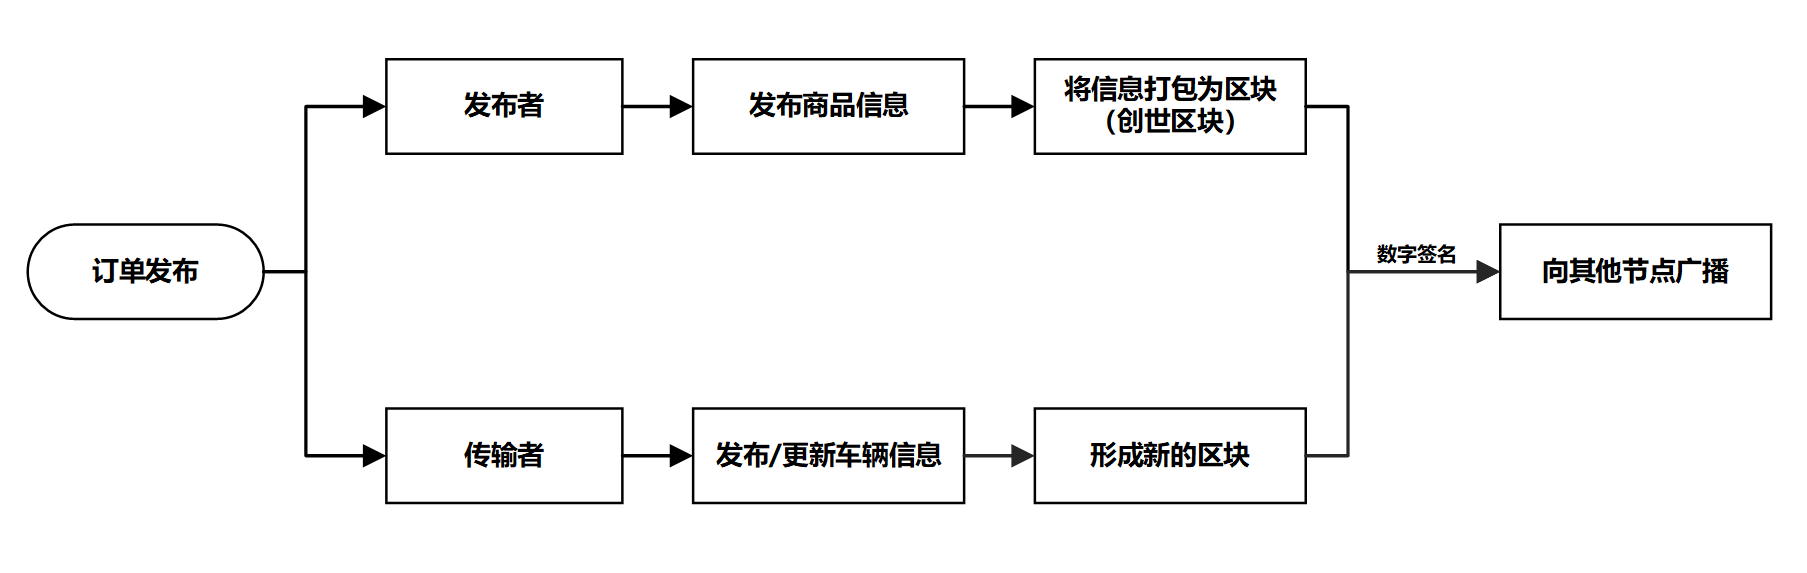
\includegraphics[width=1.1\linewidth]{image/order.png}
    % 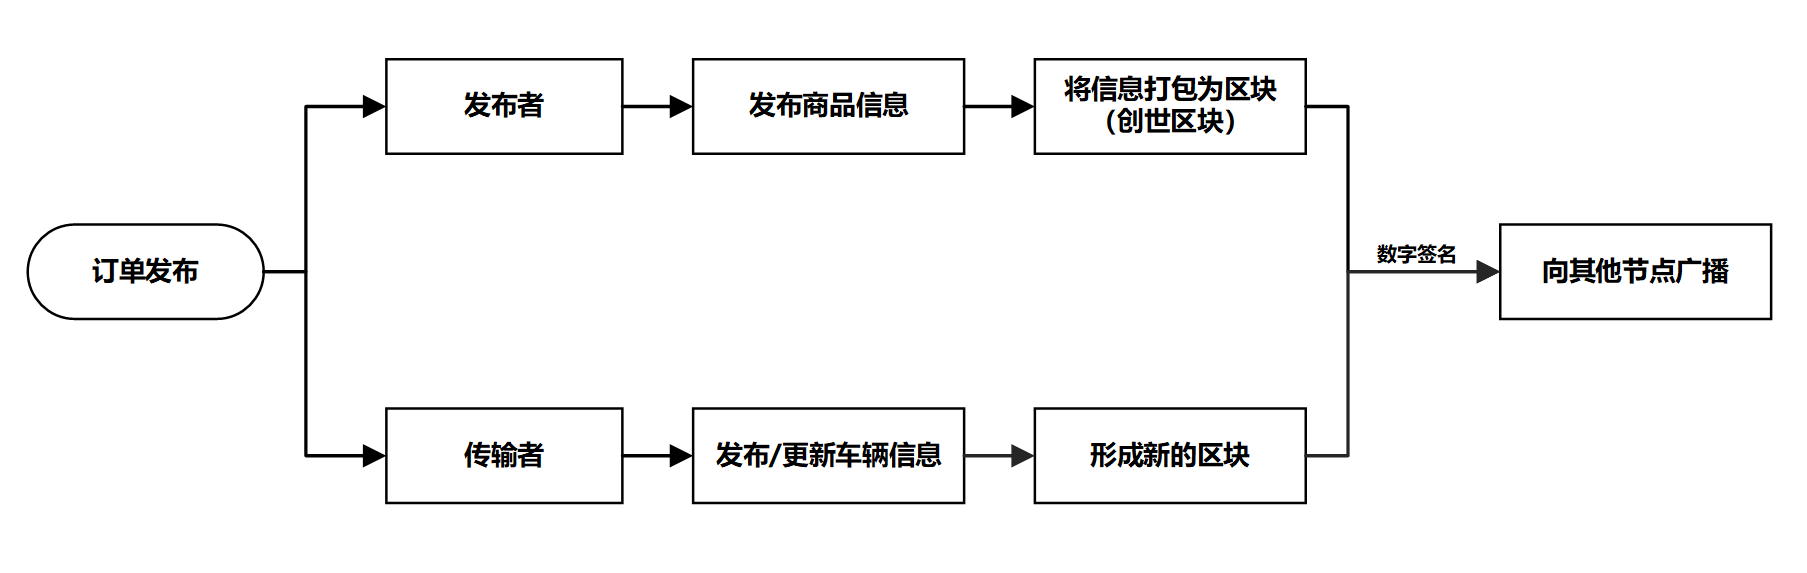
\includegraphics[scale=0.2]{image/order.png}
    \caption{\heiti\small订单发布示意图\songti}
  \end{figure}
  在订单发布后,系统后台自动运行车货匹配推荐算法。发布者可以看到根据推荐算法计算出的匹配程度由高到低的可用车主信息\footnote{这里的可用也可能指在马上执行完上一次任务的司机,且上一次任务的终点处于本次任务的起点。}。司机可向订单发布者发送接单申请,订单发布者也可以向司机发送接单申请。当另一方同意了接单申请后即进行双方即进行数字签名,将该成交订单向其他节点广播。
  \subsubsection{运输部分}
  运输部分建立在订单发布后司机已经接单的前提下,这部分可以对订单部分进行实时更新,包括检查订单状态、检查实时位置等操作。该部分流程如下。\\
  \indent 1、司机到订单指定起点位置,将要运输的货物装载。装载完成后,司机对该区块链上的运输信息进行数字签名,广播到其它节点。一旦检测到该过程结束,系统便会会这个订单生成一个用户的查询接口。\\
  \indent 2、在运输过程中,定位模块将对货物的位置信息(实质上是司机的终端设备的位置信息)进行实时更新,每一次的位置操作也都将更新到区块中,形成不可更改的货物位置追踪记录。\\
  \indent 3、当司机将货物送至指定地点时,让收货人进行验收,若验收成功,则对该订单信息进行数字签名,发布并等待其他节点验证。当上述操作完成之后,该订单确认送达,进入转账操作。
  \begin{figure}[H]
    \centering
    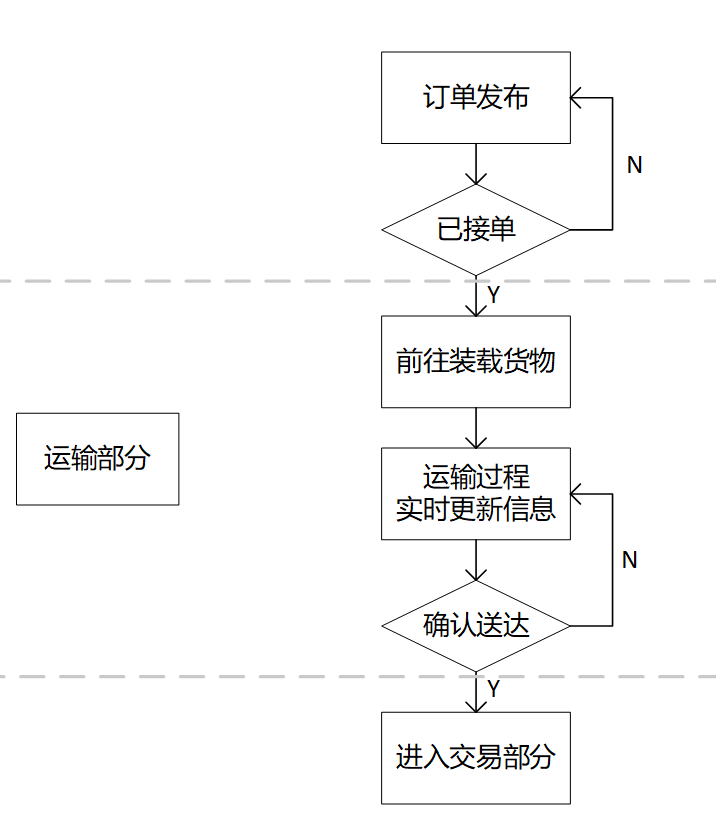
\includegraphics[scale=0.6]{image/transfer.png}
    \caption{\heiti\small运输部分流程示意图\songti}
  \end{figure}
  \subsubsection{交易部分}
  当用户确认物品已经安全送达后,系统会向发布用户提交转账申请。\\
  \indent 首先系统会判定发布者的对应的地址余额是否充足,当用户同意进行转账操作并且余额充足后,转账操作进行,订单发布者与司机账户对应余额减少或增加相应数量。转账操作结束后两个账户对此次操作进行数字签名并广播到其它节点。
  \subsection{推荐算法部分}
  该部分目的在于快速匹配与需要运送货物相符的车辆或为车辆匹配与之对应的货物订单。因此我们决定采用一种在优先满足硬性条件前提下的的基于车辆推荐的画像数据可用性判断方法结合匹配中的四种“软性条件匹配”模型\cite{ref3}——“路线匹配模型”“意愿衰减模型”“车辆靠近趋势模型”“熟车关系模型”。这些推荐算法与模型将在后文中详细说明。
  \section{区块链技术在该平台中的应用}
  如上文所说,基于EOS项目免费试用、轻松调试、低延迟、串并行性能高的特点,我们在该平台中决定使用EOS进行智能合约的部署。该部分详细介绍了该项目在如何区块链上的部署与执行。
  \subsection{EOS介绍}
  \indent EOS和ETH的愿景大致相似,都是一个操作系统的底层。其中我们可以构建各种各样的智能合约应用。而EOS通过并行链和DPoS的方式解决了延迟大,和数据吞吐量小的难题。EOS的数据吞吐量理论可以达到百万TPS的数量级。该区块链不需要通过费用来加入与执行合约,大大降低了部署与运行的成本。\\
  \subsection{EOS账户}
  EOS自带基于角色权限管理和账户恢复功能的账户体系,是一种更加灵活的组织和管理账户的方式。EOS.IO软件允许帐户可被长度多达12个字符的唯一可读名称所引用。该名称由帐户的创建者选择。帐户创建者必须保留存储新帐户所需的RAM,直至新帐户存储令牌以保留其自己的RAM\cite{ref4}。EOS没有采用地址的形式而是采用账户的形式,这是EOS相对于以太坊和比特币的不同之处。每一个账户都为长度为12位\footnote[1]{事实上可以存在小于12位的账号,但长度小于12位的账号属于高级账号,系统每天进行只会进行最多一次高级账号的拍卖。如第一个拍卖的账户名"eos"价格高达50000EOS,现在价格已超过百万人民币},包含了英文字符'a'$\sim$'z'以及数字1$\sim$5,这样的优点在于将原来没有固定格式的长地址形式转换为人们容易记住的形式。\\
  \indent 重新回到考虑如何在我们设计的平台中使用EOS的优势来进行部署的问题。EOS账户中自带两个权限:owner与active\footnote[2]{还存在一个账户被盗后用于恢复账户的Recovery权限与用户自定义的权限,我们在这里不做考虑}。两者实质上都是私钥的形式。Owner权限代表了用户对账户的所有权,可以对账户进行任何修改。而active权限一般用于转移资金、执行智能合约、为DPoS机制中的区块生产者投票等等操作。事实上在EOS系统中智能合约也有类似的权限,我们在实现该运输平台的合约时便可运用这一特点。具体的说,我们可以在合约权限中设置阈值,每当有新的订单发布或转账操作要进行,我们就让该系统中所有账号进行验证,只有当最后认可该信息的节点数量大于事先设定的阈值时,该信息才最终会被更新到作业链上。通过这样的方式,我们可以确保数据的安全性以及真实性。\\
  \subsection{数字签名}
  在上文提到了其他节点用于验证信息真实性、确定身份、确定责任的方法便是数字签名,几乎全部区块链项目都采用了数字签名这一方法,EOS也不例外。在我们的系统中并不需要我们自己来构建数字签名的加密算法,但其作为几乎作业链中每一个流程都需要用到的东西,我们决定在这里介绍一下EOS中数字签名的过程。\\
  \indent 在上一小节中提到了EOS账户,而这一节中我们则介绍与之相对应的“钱包”。在EOS系统中,钱包与账户并不一一对应,相反它们可以存在一对多的关系,即一个钱包中可以管理许多账户,而这里账户的表现形式形式便为私钥。其关系可参照下图3。\\
  \begin{figure}[H]
    \centering
    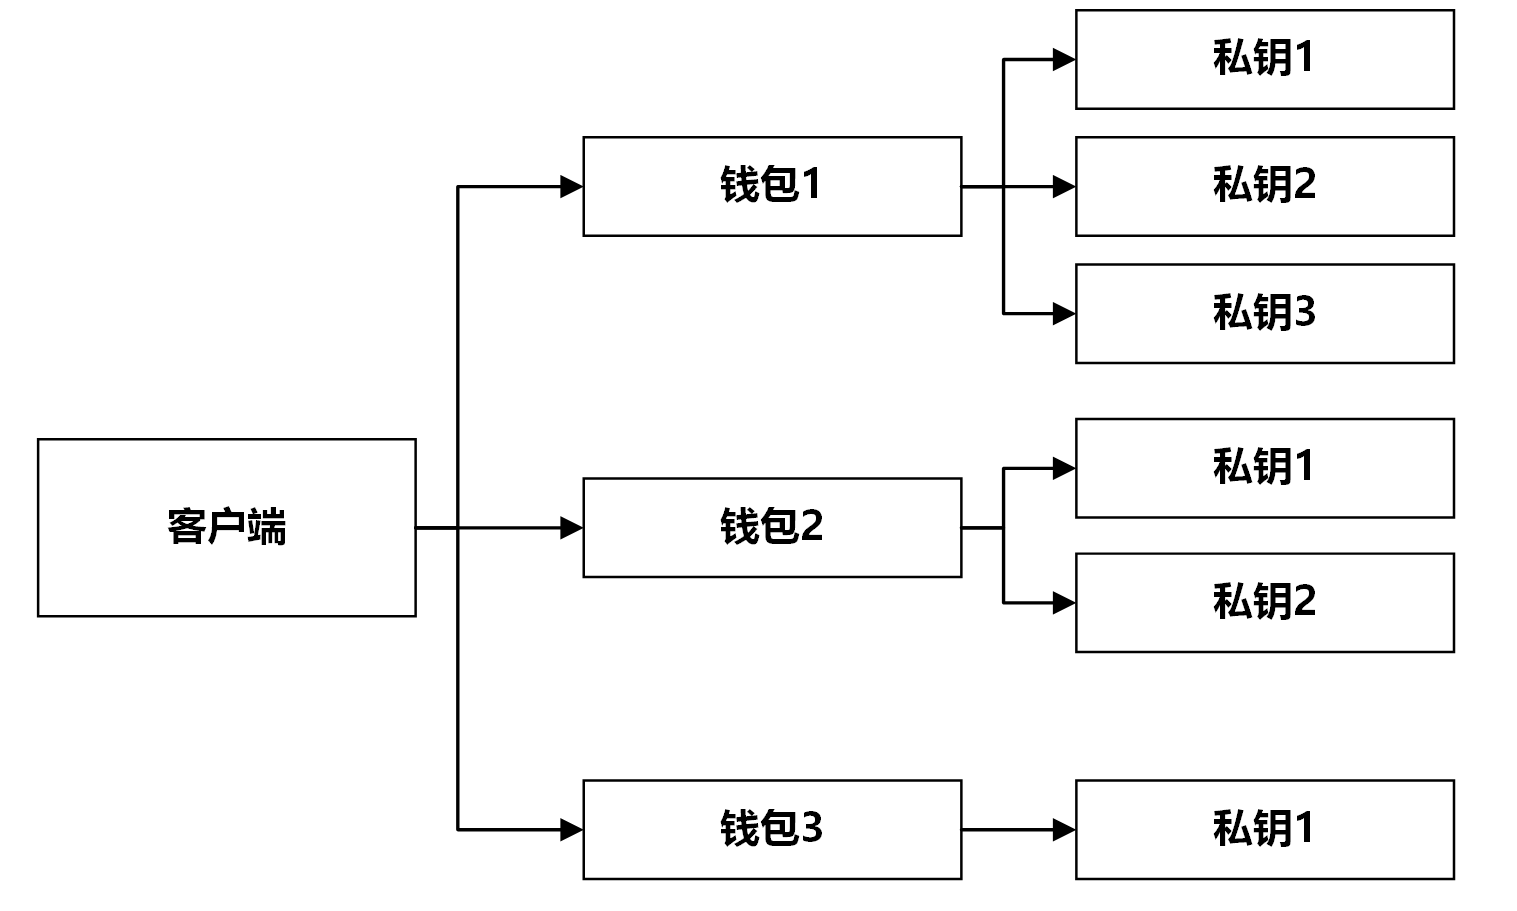
\includegraphics[width=\linewidth]{image/psw.png}
    \caption{\heiti\small钱包-私钥对应关系\songti}
  \end{figure}
  \indent 而数字签名的工作流程如图4所示。发送方对原始数据通过哈希计算数字摘要,接着使用非对称加密\footnote[1]{EOS中采用了椭圆曲线加密方式}中的私钥对其进行加密,然后将加密后的数据向其他节点广播。当接收方进行验证时,首先使用发送者公钥对数字签名进行解密,将原始信息的散列值与解密出的散列值对比,只有两者相同时签名验证才算通过。
  \begin{figure}[H]
    \centering
    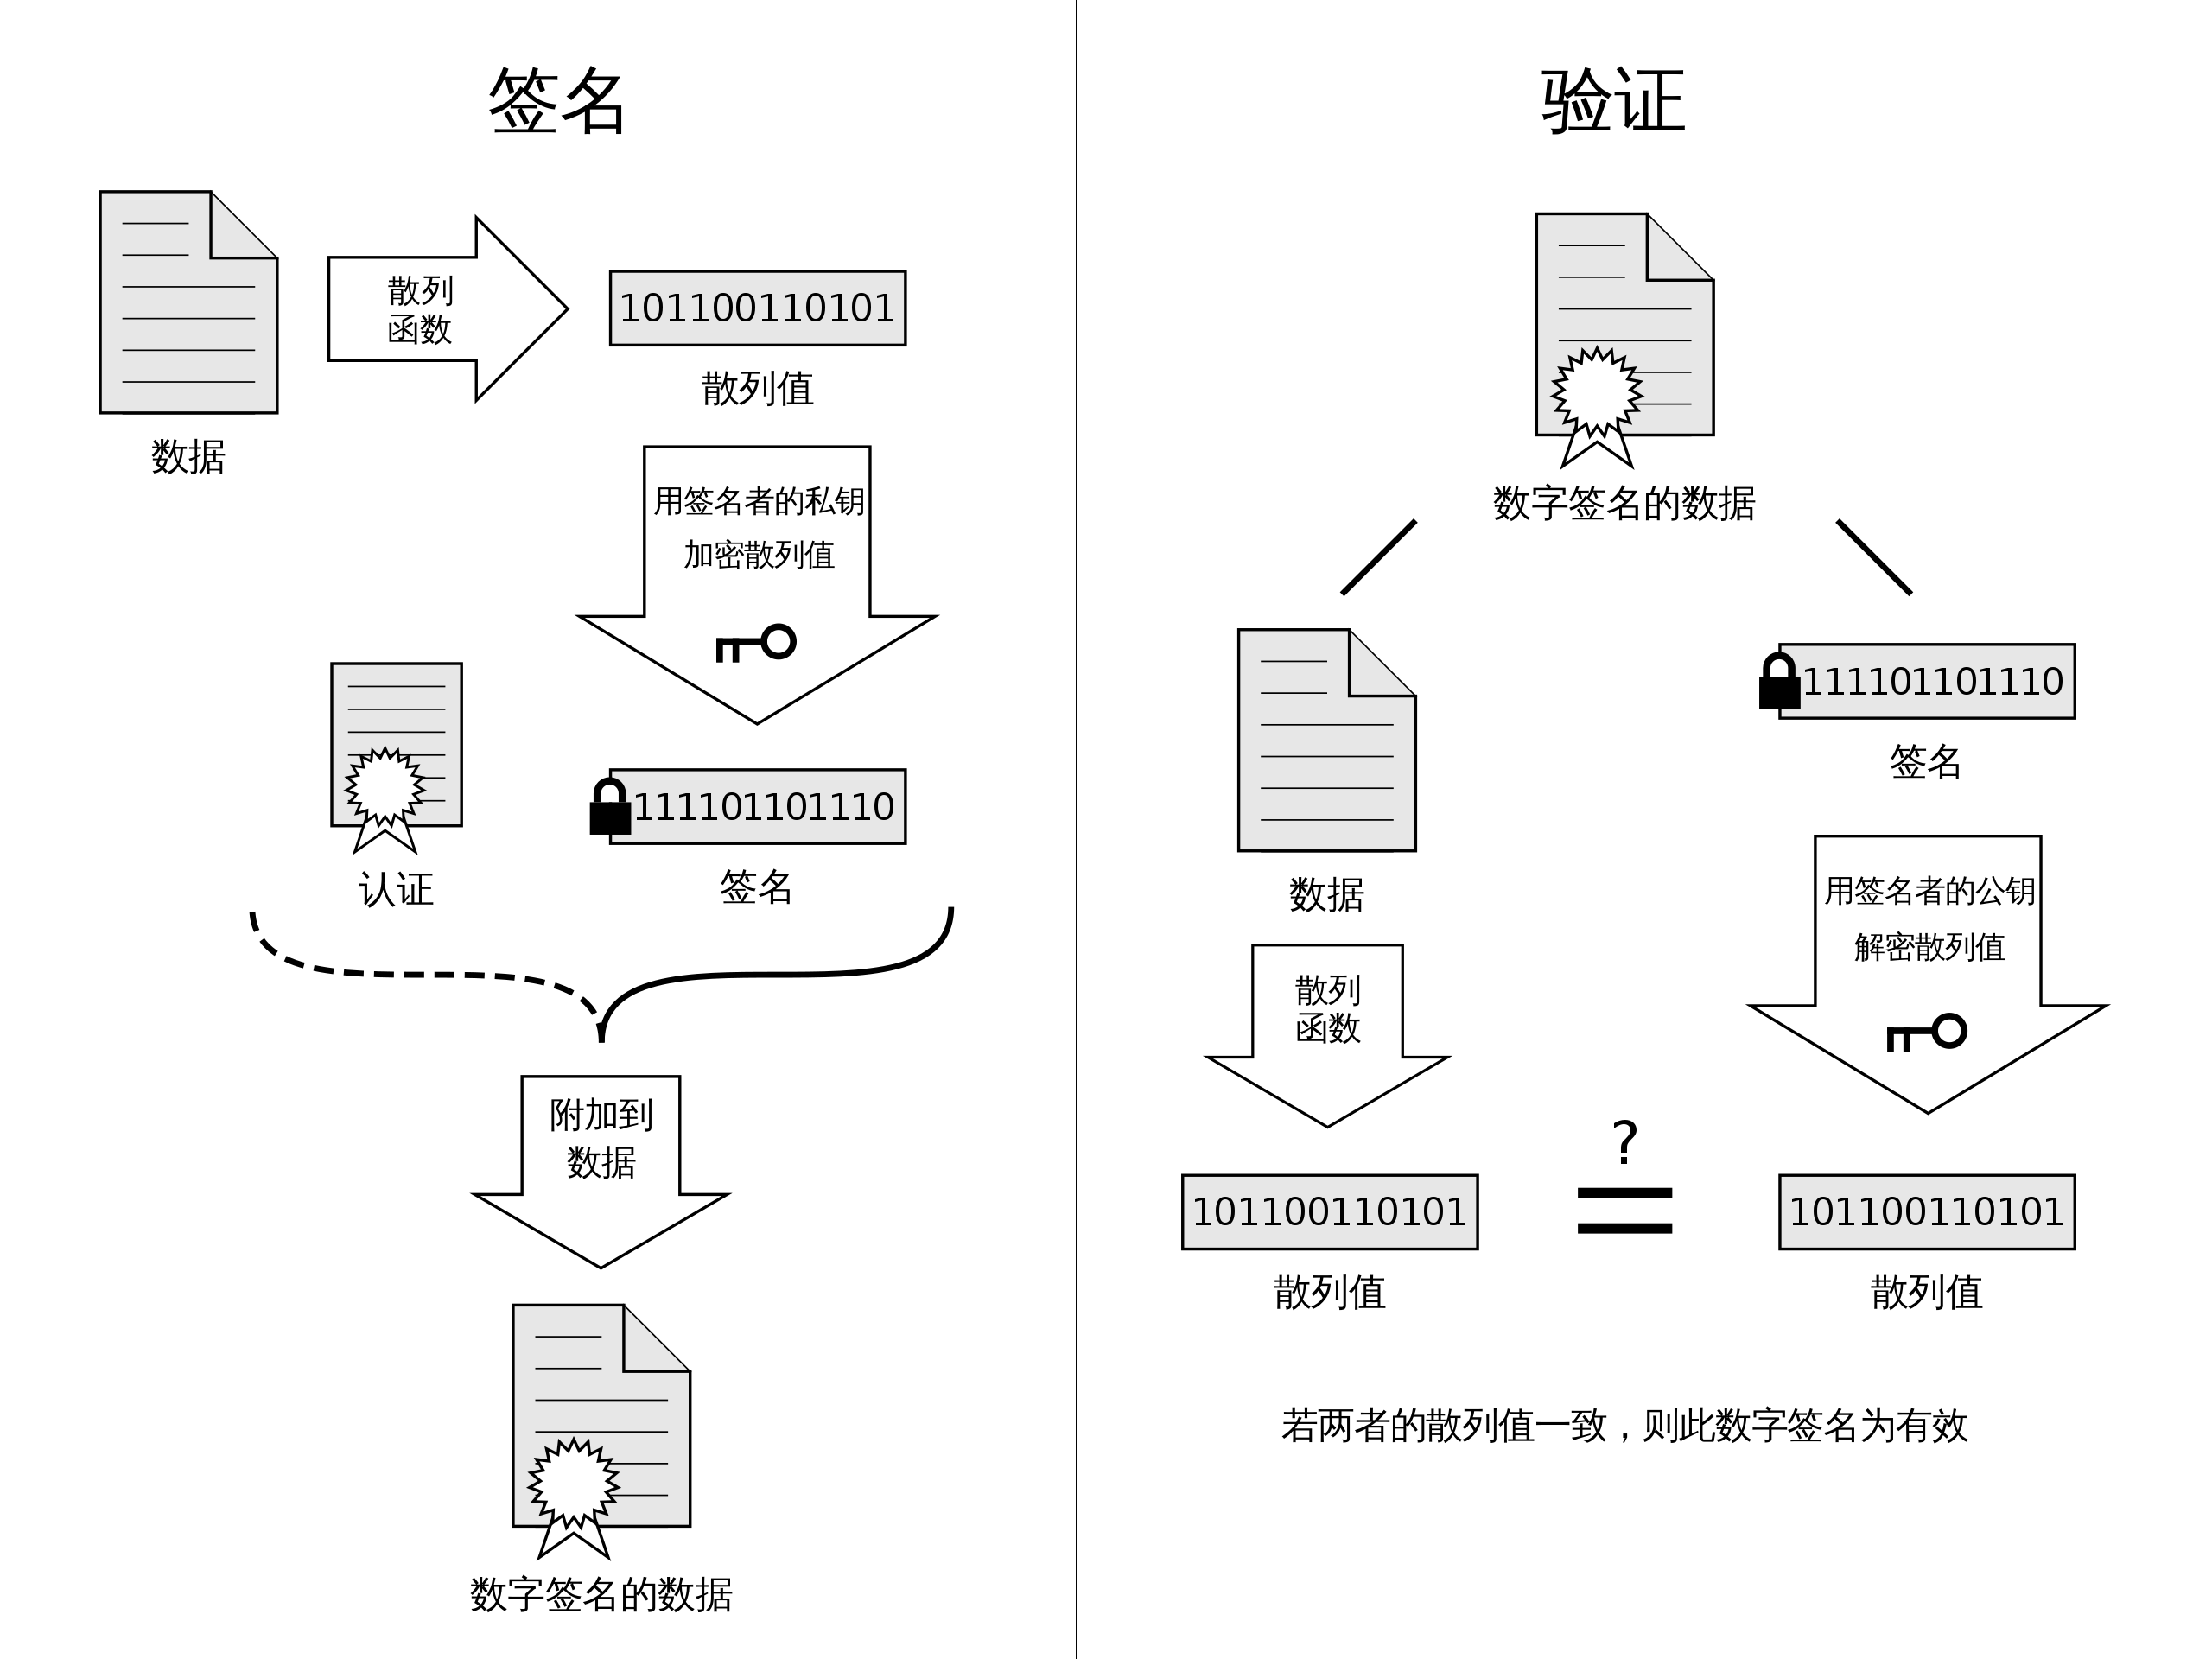
\includegraphics[width=\linewidth]{image/check.png}
    \caption{\heiti\small签名及签名验证的流程示意图\songti}
  \end{figure}

\section{IPFS在该平台中的应用}
\subsection{IPFS介绍}
IPFS(星际文件系统,Inter Planetary File System)是一个旨在创建持久且分布式存储和共享文件的网络传输协议。它是一种内容可寻址的对等超媒体分发协议。在IPFS网络中的节点将构成一个分布式文件系统。\\
\indent在本地IPFS 系统中的文件存在两种状态,分别为永久存储和缓存状态,使用PIN功能可以使永久存储状态和缓存状态互转换。IPFS 系统的寻址方式分为两种,一种是IPFS寻址(不可变内容寻址),由梅克尔有向无环图提供的基本内容寻址;还有一种是SIHPNS寻址(可变内容寻址),即节点将IPFS 数据发布到每个IPFS 节点的不可更改的IPFS 地址下,从而达到可变内容寻址的目的。
\subsection{应用与分析}
根据EOS白皮书的介绍,EOS将来会内置一个IPFS标准的文件系统\cite{ref5}\\
\indent 我们希望基于EOS开发货物传输平台,而EOS的交易量非常大, 0.5s会产生一个区块的数据。如果所有用户信息与交易数据全部记录在主链上,那么将会产生非常巨大的数据量,而通过IPFS可以极大地降低主链本身的数据存储成本。\\
\indent 此外,DApp在用户访问前端时需要静态的页面分发服务,它的前端文件目前是中心化的。通过把这些前端程序或者网站前端放到基于IPFS的文件存储上,只需要抵押一定的EOS代币,就可以实现Web服务的去中心化和低成本。\\
因此,我们可以将账户系统与交易系统放在EOS 主链上,将前端页面、车辆信息、司机信息、路线信息等信息、推荐算法和预处理信息等全部放在IPFS 上,确保低成本的同时进行了完整的体系架构。\\
\indent 而相比传统的数据中心化、难备份的储存方式,IPFS能够永久的、去中心化保存和共享文件,从而使我们的交易记录和用户信息全部得以永久安全储存,且便于我们查询溯源 ;在传统的数据存储中,数据是被直接储存的,安全性并不让人满意,而IPFS会对所有内容都进行加密与校验。我们通过EOS实现一个文件交易DApp,那么所有文件便可以通过IPFS存储,并用密钥加密来保证其安全性,用户也可以通过修改密钥可实现链上的产权转移达到文件交易的目的。此外,相比于传统的区块链,IPFS并不会要求每一个节点都存储所有的内容,节点的所有者可以自由选择想要维持的数据,在备份了自己的用户与交易数据之外,可以自愿的为其他的用户提供数据存储服务并从中活动利好,解决了传统区块链区块数据量巨大而每个节点都必须全部下载的痛点。













%   \section{信用评估和准入规则}
%   \begin{table}[H]
%     \centering
%     \begin{tabular}{|c|c|}
%       \hline
%       $C_0$ & 被推荐用户初始信用 \\ \hline
%       $C_p$ & 推荐者的信用 \\ \hline
%       z &被推荐者的芝麻分\footnotemark[2]\\ \hline
%       $C_p^{'}$ & 被推荐者初始信用 \\ \hline
%       x & 用户评分 \\ \hline
%       N & 同时接受订单数量 \\ \hline
%     \end{tabular}
%   \end{table}
%   \footnotetext[2]{支付宝提供了芝麻分查询的接口,这不但可以实现信用的评估,还可以实现一人一个账号的限制功能。}
%   \picfig{表格1 \ \ 信用评估与准入}
%   \subsection{信用评估方式}
%   \subsubsection{初始值}
%   \indent 推荐制是由原用户推荐,新用户得以加入的机制。推荐制进入的用户虽仍要在接单时缴纳押金,但是将享有特别的福利,此环节将在“动态评估”部分讨论。
%   \indent 通过推荐制成为外卖员的用户,初始的信用分将由推荐者的信用、被推荐者的支付宝芝麻分决定:
%   $$C_0=0.3 C_p + 0.7 \times \frac{z}{950} \times 100$$
%   \indent 押金制原指客户在买卖期货时需缴纳相当于合同价值一定比例的押金,在这里指的是通过缴纳一定的押金作为保证金,作为用户初期信用与消费者权益的保证。\\
%   \indent通过押金制成为外卖员的用户,初始的信用分数将由其支付宝芝麻分决定,公式如下:
%   $$C_0=\frac{z}{950} \times 100$$
%   \subsubsection{动态评估}
%   对于推荐制,推荐者初始每人有3个推荐名额,且推荐者的信用分将会受到被推荐者的影响:
%   $$C_p^\prime=C_p-\ln(\frac{C_0}{65})\times e^2$$
%   \indent 随着信用值的上升,推荐者将获得更多的推荐名额n:
%   $$n=\lfloor 3+\frac{C_p-65}{187} \rfloor ,(n \leq 10)$$
%   \indent 而被推荐者也将享受到推荐制的福利,被推荐后将享有5单的免押金订单的机会,且将获得信用积累加成:
%   $$\mathrm{\Delta C}^\prime=(1+\frac{10}{x_t} )\mathrm{\Delta C}$$
%   \indent 而对于一般用户,每当用户完成订单且获得好评(4星/5星)时,其信用分C就能提升$\Delta C$
%   $$\Delta C=\left\{
%     \begin{array}{lr}
%     \frac{x-3}{5} N, & {N \leq 5} \\
%     \frac{x-3}{5} N + \frac{x-3}{5}\times \frac{3N-15}{N} ,& {N > 5}
%   \end{array}\right.
%   $$
%   \indent 如果获得中评,则信用积分不发生改变;\\
%   \indent 但如果获得了差评(1星/2星)时,其信用分C就会下降$\Delta C$
%   $$\Delta C=\left\{
%     \begin{array}{lr}
%     \frac{x-3}{5} N, & {N \leq 5} \\
%     \frac{x-3}{5} N + \frac{x-3}{5}\times \frac{3N-15}{N}, & {N > 5}
%   \end{array}\right.
% $$
%   \indent 其中x为用户评分,N为同时接受的订单数。此处限制了骑手同时接多单所获得的信用值,是为了避免骑手所接单数超出其能力范围而导致延误的情况再度出现。\\
%   \indent 但当订单出现较大的事故(收到顾客投诉等情况)时,经核实后将会扣除△C的信用,并且此后所接五单价值无法超过30元。
%   $$\mathrm{\Delta C}=-\left(100+\frac{c_0}{10}\right)$$
%   \subsubsection{信用等级制度}
%   \indent 信用是衡量一位外卖员诚信度与活跃度的重要指标。用户成功完成的订单数越多,信用将会越高,反之当出现丢单或延误等顾客投诉的情况,用户信用将较大幅度降低。\\
%   \indent 信用的最大值为1000。每100分为1等级,且用户凭借等级lv能够获得押金减免D:
%   $$lv=\lfloor \frac{C_0}{100}\rfloor$$
%   $$D=10lv$$
%  同时,信用等级高的用户将获得额外的分红:
% $$\Delta m=\frac{lv}{20}\times\ \Delta m_p$$
% 其中$\Delta m_p$是平台在此单中获得的收益。
%
%   \subsection{准入规则}
%   \subsubsection{推荐制}
%   \indent 本平台使用的推荐制是通过原本平台内的正式外卖员参与,经过他们的推荐与信用评估来完成新外卖员的纳新,但新外卖员的信用水平会一定程度上影响推荐者的信用水平。被推荐并通过评估的外卖员将成为正式外卖员,不需要提交押金即可进行接单。\\
%   \indent “供求关系”是经济学的基石, 是指在商品经济条件下, 商品供给和需求之间的相互联系、相互制约的关系。外卖平台对优秀外卖员的争夺, 类似于商品经济中对商品的追求。“接收”平台相当于“买方”, 推荐用户相当于“卖方”, 新进外卖员则是推荐用户生产的“商品”。某一被推荐的外卖员, 热爱工作、积极进取, 则在市场上处于“供不应求”的地位;反之, 平台自身对外卖员待遇差, 优秀的外卖员自然不愿意与此平台签订合约, 必然导致“供大于求”。\\
%   \indent 基于“供求关系”的分析可知, 推荐资格、推荐名额的分配, 以及接收推荐外卖员的比例, 应交由“市场需求”自主调节, 充分发挥“市场”调节的效率, 高效准确地选拔出优秀的外卖员。通过“市场”的优胜劣汰, 激发平台自身的发展潜力, 一方面, 推荐用户会高度重视自身的相关利益, 谨慎决定推荐数量与对象, 培养出符合平台需求的优秀外卖员。另一方面, 平台也会不断为新进外卖员提供优质的接单渠道等, 吸引更多的外卖员加入。
%   \picturehere[0.4]{image/tree.png}
%   \picfig{图4  \ \ 推荐制示意图}
%   \subsubsection{押金制}
%   \indent 本平台使用的押金制是等价抵押机制。非正式骑手可以通过提交与所接单价值等价的金额来完成接单,并在订单完成后与报酬一同汇入非正式骑手的账户中。随着此类订单完成次数的增加,非正式骑手的信用值会相应增加,随着信用值增加骑手所需缴纳的押金会逐渐减少,而信用值到一定程度后可申请成为正式骑手,此后接单将不再需要押金。\\
%   \indent 押金能有效地保障消费者的权益,降低交易费用,从而保障交易安全。押金的存在避免了部分新进外卖员偷餐、毁坏订单等举动后销号退出的逃避后果的行为,是外卖员前期信用保证的辅助制度。
%   \subsubsection{实际结合方案}
%   经过讨论,我们发现,两种方法单独使用均无法达到使平台健康发展的目的,仅使用推荐制会导致骑手数量无法扩张且无法实现“人人都有机会参与”的初衷;而仅使用押金制则无法树立平台的诚信,常常被误认为是诈骗,而导致平台成立初期无法发展。\\
%   \indent 因此本平台最终使用的准入规则是推荐制与押金制并行、分级准入的准则。\\
%   \indent 在平台发展的初期,无法获得足够的人力,而押金制在信用建立的前期很难推行。故在平台开设初期应先招募一批愿意参与试运行的外卖员,先由他们通过试单来体验平台的收益,并通过推荐制来招募新的人员,此时推荐制的信用激励机制则起到了助推的作用。在平台的信用建立起来之后,再逐步形成以押金制为主,以推荐制为辅的运行方式。通过学号+电话号码的验证机制与初始信用分的评估机制,每一位学生都有机会通过上述两种方式参与到代送外卖的交易中,并随着参与次数与推荐成员的增加获得更多的福利,进而使更多学生参与到本平台中。由此,外卖由于人手不足导致的送餐延误将会大大减少。
%
%
%   \section{延时保险模型}
%   \begin{table}[H]
%     \centering
%     \begin{tabular}{|c |c|}
%       \hline
%       R               & 期望骑手费用           \\ \hline
%       S               & 订单金额           \\ \hline
%       $R^{*}$         & 系统计算骑手费用最小值           \\ \hline
%       $t_1$           & 商家出单时间           \\ \hline
%       $t_1^{*}$       & 系统计算商家出单时间           \\ \hline
%       $t_2$           & 骑手送餐时间       \\ \hline
%       $M_s$           & 返回商家金额           \\ \hline
%       $M_t$           & 返还骑手金额           \\ \hline
%       $M_c$           & 返还顾客金额           \\ \hline
%       $\alpha,\beta,\gamma,\sigma$           & 赔付系数(在正文中解释)           \\ \hline
%     \end{tabular}
%     % \caption{}
%   \end{table}
%   \picfig{表格2 \  延时保险赔付模型}
%   \subsection{用户下单}
%   用户下单金额为$S$,期望骑手费为$R(R>R^{*})$,期望时间为$T$,用户需往平台中充入$S+R$。
%   \subsection{商家接单}
%   商家接单后需往平台中充入$R×\alpha(\alpha>1)$,出单时间为$t_1$(容忍时间为$t_1^{*}$)。
%   \subsection{骑手接单}
%      骑手接单后需往平台中充入$S×\beta(\beta>1)$,送达时间为$t_2$。
%   \subsection{送达情况}
%   \indent 送达后,则进行返还押金与分配利润的步骤。
%   \subsubsection{成功送达}
%     \indent下面讨论用户购买了延时保险的情况。 \\
%     \indent 对商家有:
%     $$
%     M_s=\left\{
%       \begin{array}{lr}
%         R \times \alpha + S,  & {t_1 \leq t_1^{*}}\\
%         R \times \alpha \times f(t_1-t_1^{*}) + S \times \gamma, & {t_1 > t_1^{*}}
%       \end{array}\right.
%     $$
%     \indent 对骑手有:\\
%     \indent令$$T_{md} = S \times \beta $$
%     $$ G_{md}=R \times g(t_2-T+t_1^{*})$$
%     \indent 则
%     $$
%     M_t=\left\{
%       \begin{array}{lr}
%         T_{md}+R,  & {t_2 \leq T-t_1^{*}}\\
%         T_{md} + G_{md} + S \times \gamma, & {t_2 > T -t_1^{*}}
%       \end{array}\right.
%     $$
%     \indent 对用户有:若$t_1+t_2>T$,则将合约内与该订单相关的钱悉数退回。
%   \subsubsection{丢单}
%
%   \indent 对商家有:
%   $$M_s=R \times \alpha $$
%   \indent 对骑手有:
%   $$M_t=S \times \beta \times \sigma$$
%   \indent 对用户有:
%   $$M_c=(1+\alpha)\times R +(1+\beta)\times S    -M_s-M_t$$
%   \subsubsection{无人接单}
%   \indent 用户可选择提高$R$以吸引其他骑手接单,或者选择取消订单,但需要支付一定的赔偿与手续费用于赔偿商家的损失。
%   \subsection{赔付系数}
%   \indent 这里我们令$h(n)$为单位次数商家发生延迟的比率,$p(m)$为单位次数骑手延迟的比率。\\
%   \indent 再令:$$E(n)=1-e^{- \int_{0}^{n}h(n)dn}$$
%   $$F(m)=1-e^{- \int_{0}^{m}p(m)dm}$$
%   \indent 则以上系数$\alpha, \beta$ 分别可以表示为:
%   $$\alpha = \frac{E(n)+E_A}{E_A}$$
%   $$\beta = \frac{F(m)+F_A}{F_A}$$
%   \indent 另外的$\gamma$则决定的是成功送达时平台的盈利系数,其与骑手用户的信用等级、订单金额等因素均相关,且在平台不同阶段均会产生改变,暂设定为人为改变系数,这里不做讨论。\\
%   \indent 而$\sigma$则是丢单时骑手应赔付的金额,这与通知用户丢单的时间造成的时间损失与用户订单的金额相关,同时视外界环境因素(如恶劣天气)影响,这里也暂不做讨论。
%
% \section{完备性与缺点分析}
% \subsection{完备性分析}
% \indent 下面将经由与传统校园外卖模式的对比阐明本模型的完备性。\\
% \indent 其一,现有校园外卖系统普遍缺少延时险功能,难以基于外卖延误等问题对消费者进行赔偿。该模型运用智能合约平台提供了完善的延时险机制,可以有效地对消费者进行补偿。同时,商家和骑手双方面临的补偿金额,也能在一定程度上引起他们对于配送效率和配送安全的重视,减少校园内送餐拖延事件的发生。\\
% \indent其二,我们看到,即使一些全国大型外卖平台提供了相应的延时险服务,但是目前的外卖延时险制度细则和标准各不相同,具体实践存在差异。同时由于在传统的延时险赔偿中,监管者往往处于被动监管地位,消费者处于弱势地位,外卖企业对于延时纠纷的判定从主观上更加倾向于自身利益。基于智能合约的延时险赔偿机制则可以做到判定的公平,从客观上消除企业对消费者这种隐性的利益损害。\\
% \indent其三,目前的外卖信息管理都是中心化的,外卖企业对于外卖配送数据处于支配地位,客观上存在数据篡改、数据伪造等可能,从而影响纠纷判定。这种情况将在很大程度上导致消费者对外卖平台、商家的不信任以及对现有外卖延时险机制的不满,同时也增加了监管者对纠纷的监管难度。我们通过搭建去中心化的平台,客观上去除了数据篡改与伪造的可能性,智能合约代码公开的特性也一定程度上解决了平台与消费者、商家与消费者之间的信任问题。\\
% \indent其四,区块链不可篡改的特性极其适用于配送流程追溯领域,其引入使得外卖过程中的数据更具备真实性。并且在区块链上,触发延时险赔偿的原因细节、赔付资金流向等信息能够实现公开透明,打破外卖企业与消费者之间的信息不对等,进一步维护消费者权益。\cite{fuck}
% \subsection{缺陷分析}
% \indent到目前为止,我们的模型优化了现有的校园外卖系统,但是对于该平台本身来说,它在外卖延时险服务中往往只能接受来自消费者的反馈,无法主动参与监管,处于间接监督的位置。换句话说,只有当延时行为发生,平台才能做出相应的反应。为了更加主动更有效率地监督外卖配送业务,信息化的管理便必不可少,新的监管方式和技术手段也必须运用到外卖配送领域,将外卖配送中的关键环节记录下来,在保证商业隐私地情况下做到公开透明,以便减少“外卖事故”的发生。\\
% \indent另外,由于智能合约一经部署便无法进行改动,所以平台本身将面临调整与修复上的困难。其中许多参数需要随着时间与经营环境的改变进行调整,以便适应市场变化;同时,考虑到平台可能存在难以发现的漏洞,在未来时时面临着被漏洞攻击的可能性,我们也需要根据情况对智能合约进行修改与完善。无论是调整还是修复,都需要将更新后的合约重新部署到区块链上,而平台与合约之间的接口也需要随着合约地址的改变而改变,这些都将促成维护成本的上升。
% \subsection{与传统模式的对比}
% \picturehere[0.55]{image/advance.png}
% \picfig{图5  \ \  改进模型对比}
%
%
\end{multicols}
%
\renewcommand{\refname}{参考文献}
\bibliographystyle{unsrt}
\bibliography{bib}
\end{document}
